\section{Launcher}
The launcher is the part of the eclipse framework responsible to "launch" the code to run, in our case a model to be interpreted. Associated with a launch is a launch configuration that contains information used to launch the code. The inspiration for the Overture implementation can be found \href{http://www.eclipse.org/articles/Article-Launch-Framework/launch.html}{here}\footnote{\url{http://www.eclipse.org/articles/Article-Launch-Framework/launch.html}} \cite{Szurszewski03}. 
Also connected with the launcher is its UI part which is the window that pops up when a defining a new launch configuration.

\subsection{The players}

\begin{description}
\item[launchConfigurationType:] it is an extension point where new launch configurations can be declared. A launch configuration describes a way to launch a model; 

\item[launchConfigurationDelegate:] it is a delegate associated with a launchConfigurationType. The delegate is in charge of, using the configuration set for launch, starting up the interpreter process. The configuration contains which is the launch mode (i.e. "run", "debug") among other settings;

\item[launchConfigurationTypeImages:] it is an extension point to select an image associated with a launch configuration type;

\item[launchConfigurationTabGroups:] it is an extension point that defines a tab group associated with a certain configurationType. The tab group is a group of tabs presented when creating a new launch configuration which contain the enables the user to graphically set the settings to be used in the launch (configuring it);

\item[launchShortcuts:] it is an extension point that enables the definition of shortcuts to launch models without configuring the launch, i.e. without bringing up the launch configuration tabs.

\item[launchGroups:] didnt get there yet... not sure if it will be needed.

\end{description}

\subsection{launchConfigurationType}
To define a new launchConfigurationType this is the extension point.

\lstset{language=XML, caption=lauchConfigurationTypes extension point}
\begin{lstlisting}
 <extension
         point="org.eclipse.debug.core.launchConfigurationTypes">
      <launchConfigurationType
            delegate="org.overture.ide.debug.core.launch.VdmLaunchConfiguration"
            id="org.overture.ide.debug.launchConfigurationType"
            modes="run, debug"
            name="Overture Launch Configuration Type"
            public="true">
      </launchConfigurationType>
   </extension>
\end{lstlisting}

Important fields here are the
\begin{description}


\item[delegate:] a class that implements \class{ILaunchConfigurationDelegate}. The \class{VdmLauchConfigurationDelegate} is located in the package \epoint{org.overture.debug.core.launching} and it contains the code that checks the given configuration and that launches the interpreter thread;

\item[delegateName:] humman readable name for the delegate;

\item[id:] a suitable "id";

\item[modes:] the modes which the launcher support, in our case: "run" without debug and debug mode;

\item[name:] the human readable name for the configuration;

\item[public:] setting this attribute to true enables the launch configuration to be presented in the UI;

\item[sourceLocatorId:] we will come back to this attribute later in the debug section;

\item[sourcePathComputerId:] same as the one above.
\end{description}

There is only method to be written with the launch configuration, in the \class{VdmLauchConfigurationDelegate} and it is the  method \java{launch}.
\lstjava{Snippets of VdmLauchConfigurationDelegate}
\begin{lstlisting}
public void launch(ILaunchConfiguration configuration, String mode,
    ILaunch launch, IProgressMonitor monitor) throws CoreException {
	 ...
	 }
\end{lstlisting}

The arguments are:
\begin{description}
\item[configuration:]  the configuration that the user selects in the UI is passed to the launch delegate through this variable;

\item[mode:] the mode in which the interpreter is supposed to run;

\item[launch:] created process and debug targets are added to this variable;

\item[monitor:] UI progress monitor of the launch;
\end{description}

In the \java{launch} method, the first thing to be done is to check if the actual configuration is correct. After these checks, the interpreter process is launched, if the debug mode is selected then the process should be attached to the debug target.

\lstjava{Snippets of VdmLauchConfigurationDelegate}
\begin{lstlisting}
public void launch(ILaunchConfiguration configuration, String mode,
	ILaunch launch, IProgressMonitor monitor) throws CoreException {
	
	// initial checks
	...
	// building process string
	String commandLine = "java.exe -cp vdmj-2.0.0.jar" + ...;
	...
	if (mode.equals(ILaunchManager.DEBUG_MODE)) {
		// start intepreter in debug mode
		commandLine = commandLine + "debug options";
		// start the debugger
		Process process = Runtime.getRuntime().exec(commandLine);
		// attach process to debug target
		IProcess p = DebugPlugin.newProcess(launch, process, path);
		IDebugTarget target = new VdmDebugTarget(launch,p,s);
		launch.addDebugTarget(target);
		}
	}
\end{lstlisting}
This is the simplified version of the launch delegate, in practise, because the Vdm interpreter tries to connect via a socket to the IDE when executed in debug mode, we have to start a socket server before launching the process.


\textbf{Tip 1:} the launch configuration (\java{configuration}) is still accessible while the debugger is running via the DebugPlugin. It is possible to set attributes that can be used later in the debug.
\lstjava{Changing the configuration}
\begin{lstlisting}
	...
	ILaunchConfigurationWorkingCopy workConfiguration = 
		configuration.getWorkingCopy();		
	workConfiguration.setAttribute("attribute","value");
	configuration = workConfiguration.doSave();
	...
\end{lstlisting}

\textbf{Tip 2:} use the constants in ILaunchManager to compare with the launch mode
\lstjava{Comparing the launch mode}
\begin{lstlisting}
	...
	if (mode.equals(ILaunchManager.DEBUG_MODE)) {
	...
	}
	...
\end{lstlisting}



\subsection{launchConfigurationTypeImages}
The \epoint{launchConfigurationTypeImages} extension point is a way to assign a icon to a launch configuration.


\lstset{language=XML, caption=launchConfigurationTypeImages extension point}
\begin{lstlisting}
<extension
         point="org.eclipse.debug.ui.launchConfigurationTypeImages">
      <launchConfigurationTypeImage
            configTypeID="org.overture.ide.debug.launchConfigurationType"
            icon="icons/cview16/overture_nav.gif"
            id="org.overture.ide.debug.launchConfigurationTypeImage">
      </launchConfigurationTypeImage>
</extension>
\end{lstlisting}




Fields:
\begin{description}
\item[configTypeID:] the id of the \epoint{launchConfigurationType} the image is used for;
\item[icon:] the icon to be used;
\item[id:] an id for this \epoint{launchConfigurationTypeImages}.
\end{description}

There is not much more to say about this extension point. After defining a \epoint{launchConfigurationType} and a  \epoint{launchConfigurationTypeImages} for it, the UI when the \textit{Debug Configurations...} button is pressed shows like in figure \ref{fig:launchConfigurationType}.

\begin{figure}[htb]
\centering
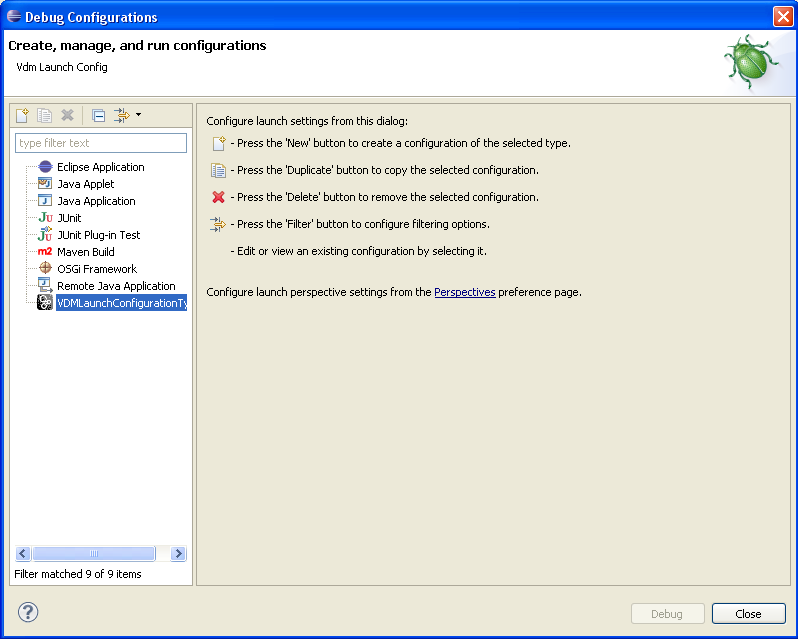
\includegraphics[width=\textwidth]{figures/launchConfigurationType}
\caption{VDM Launch Configuration}
\label{fig:launchConfigurationType}
\end{figure}

\subsection{Laucher UI part}

After defining the 2 extension points above, we have a launch type and a launch icon, but normally we would like to receive some user input (configuration) of the model to launch, such as: which is the entry point method of the model, if the user wants test coverage and so on. These options should be presented in the \textit{Debug Configuration} (figure \ref{fig:launchConfigurationType}) window when pressing our type of configuration. This is made by declaring a \epoint{launchConfigurationTabGroup}.
\begin{program}
\scriptsize
\begin{verbatim}
<extension
         point="org.eclipse.debug.ui.launchConfigurationTabGroups">
      <launchConfigurationTabGroup
            class="org.overture.debug.ui.tabs.VdmLaunchConfigurationTabGroup"
            description="Vdm Launch Config"
            id="org.overture.debug.vdmLaunchConfigurationTabGroup"
            type="org.overture.debug.vdmLaunchConfigurationType">
      </launchConfigurationTabGroup>
</extension>
\end{verbatim}
\caption{launchConfigurationTabGroup extension point}
\normalsize
\end{program}
Fields:
\begin{description}
\item[class:] the class implementing the tab group;

\item[description:] a human readable description;

\item[id:] a id for the tab group;

\item[type:] the id of the \epoint{launchConfigurationType} we want to define the tabs for.
\end{description}

Here there is also the task of defining one new class \class{VdmLaunchConfigurationTabGroup} in which only one method needs to be defined if it extends the \class{AbstractLaunchConfigurationTabGroup} class that eclipse provides.

\lstjava{createTabs method in \class{VdmLaunchConfigurationTabGroup}}
\begin{lstlisting}
	ILaunchConfigurationTab[] tabs = new ILaunchConfigurationTab[]{
				new VdmppMainLaunchConfigurationTab(mode),
				new VdmInterpreterTab(),
				new SourceLookupTab(),
				new CommonTab()
		};
		setTabs(tabs);	
\end{lstlisting}
Then the only task is to define the tabs that we would like to provide to the user. These user defined tabs should either extend the \class{AbstractLaunchConfigurationTab} or implement \class{ILaunchConfigurationTab}. Eclipse guidelines also advise to include always the \class{CommonTab} as one of the tabs and also the \class{SourceLookupTab} if we use source lookup, which will omit by now but will introduced on the debug section. The tabs defined in this class appear in the \textit{Debug Configuration} window as shown in figure \ref{fig:launchConfigurationTabs}.

\begin{figure}[htb]
\centering
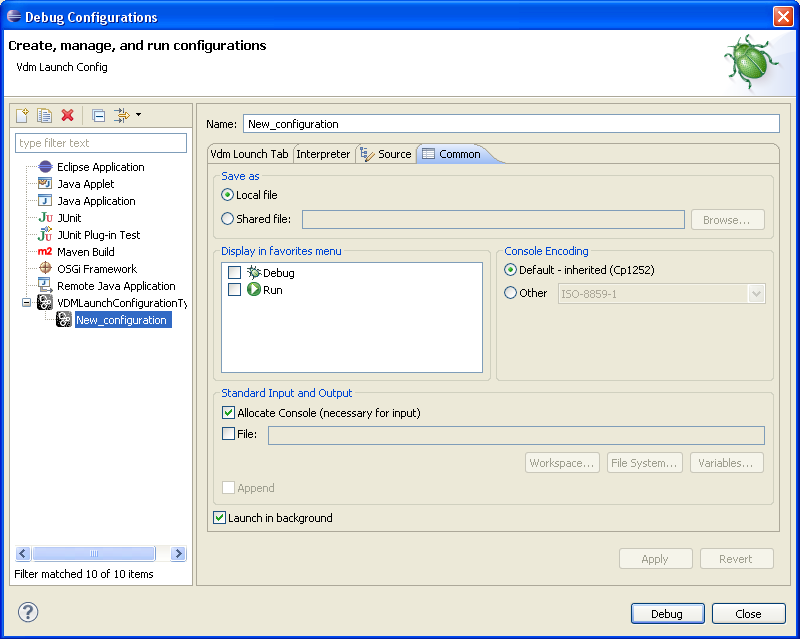
\includegraphics[width=\textwidth]{figures/launchConfigurationTabs}
\caption{VDM Launch Configuration Tabs}
\label{fig:launchConfigurationTabs}
\end{figure}

\subsubsection{Launch configuration shortcuts}
TBD.
